%!TEX root=finmath2.tex

\chapter{Репликация и оценка производных инструментов в модели Хестона}
\label{ch:hedging}
\chaptertoc

В этой лекции мы получим уравнение с частными производными для цены платежного обязательства в модели Хестона, аналогичное уравнению \bs, а также покажем, как можно реплицировать платежные обязательства, если разрешить включать в портфель дополнительные инструменты.
В третьей части лекции обсуждается метод \mc.

Несмотря на то, что все теория здесь излагается для модели Хестона, общие идеи легко переносятся на другие модели стохастической волатильности.


\section{Уравнение для цены платежного обязательства}

Рассмотрим модель Хестона и будем предполагать, что исходная вероятностная мера уже является мартингальной.
Пусть $r_t$ и $q_t$ "--- безрисковая ставка и ставка дивидендной доходности (обе детерминированные).
Тогда модель задается уравнениями
\begin{align*}
&d S_t = (r_t-q_t) S_t dt + \sqrt{V_t} S_t dW_t^{(1)},\\
&d V_t = \kappa(\theta-V_t) dt + \sigma \sqrt{V_t} dW_t^{(2)},
\end{align*}
где броуновские движения $W^{(1)}$ и $W^{(2)}$ коррелированны с коэффициентом корреляции $\rho$.

Рассмотрим платежное обязательство с выплатой $f(S_T)$.
Напомним, что инструменты с выплатой такого вида называются \emph{независящими от траектории цены базового актива}. 
Будем считать, что функция $f(s)$ ограничена снизу и $\E f(S_T) < \infty$.
Тогда безарбитражная цена этого обязательства равна
\[
U_t = e^{-\int_t^T r_s ds} \E(f(S_T) \mid \F_t),
\]
и, в силу марковского свойства процесса $(S_t,V_t)$, представима в виде $U_t = U(t,S_t,V_t)$ с функцией 
\[
U(t,s,v) = e^{-\int_t^T r_s ds} \E(f(S_T)\mid S_t=s, V_t=v).
\]

Пусть функции $r_t$, $q_t$ и $f(s)$ являются достаточно <<хорошими>>, так что к $U(t,s,v)$ применима формула \fc\ (см.~замечание \ref{sde:r:fc} в лекции \ref{ch:sde}).
Тогда получаем следующее утверждение.

\begin{proposition}
Функция $U(t,s,v)$ удовлетворяет уравнению с частными производными
\begin{align}
\label{hdg:pde}
&\prt Ut + (r_t-q_t)s\prt Us + \kappa(\theta-v)\prt Uv + \frac 12 s^2v \prtt Us + \frac12 \sigma^2v \prtt Uv + \sigma sv \Prtt Usv = r_t U,\\
\label{hgd:pde-boundary}
&U(T,s,v) = f(s).
\end{align}
\end{proposition}

Доказательство непосредственно следует из формулы \fc, применяемой к двумерному процессу $X_t=(S_t,V_t)$, который удовлетворяет уравнению $dX_t = a(t, X_t)dt + b(X_t) dW_t$ с двумерным броуновским движением $W_t = (W_t^{(1)}, W_t^{(2)})$ и коэффициентами
\[
a(t,s,v) = ((r_t-q_t)s,\ \kappa(\theta-v)), \qquad b(s,v) = (s\sqrt{v},\ \sigma\sqrt{v}).
\]

Уравнение \eqref{hdg:pde} можно решать численно методом конечных разностей.
Однако по сравнению, например, с уравнением \bs, в котором функция цены зависит только от двух переменных $(t,s)$, здесь задача становится более трудной.
Во первых, из-за присутствия трех измерений возрастает число узлов сетки, в которых вычисляется функция $U$.
Во-вторых, для неявной схемы или схемы Кранка"--~Николсона не получается применить метод прогонки, так как получаемые на каждом шаге системы линейных уравнений не являются трехдиагональными.
Если же пользоваться обычными методами решения линейных систем, то количество операций резко возрастает (напомним: для метода прогонки оно растет линейно с ростом размера матрицы, а в общем случае кубически).
В дополнении \ref{ch:adi} изложен \emph{метод чередования направлений}, который позволяет уменьшить вычислительную сложность задачи.


\section{Реплицирующие стратегии}
Так как модель Хестона не полна, то, вообще говоря, платежные обязательства в ней нельзя реплицировать портфелями, состоящими только из рискового и безрискового актива (см.~пояснение в разделе \ref{gen:s:complete} лекции \ref{ch:general}).
Репликация становится возможной, если добавить в портфель другие производные инструменты.
Покажем, как это сделать.

Нам потребуется многомерный вариант теоремы о мартингальном представлении (подробнее про теорему о мартингальном представлении в одномерном случае см.~лекцию 9 курса \intro).

\begin{proposition}[теорема о мартингальном представлении, см.~\cite{Kallenberg97}, гл.~16, теорема 16.10]
Пусть на пространстве $(\Omega, \F, \FF, \P)$ задано $d$-мерное броуновское движение $W=(W_t)_{t\ge0}$ (возможно, с коррелированными компонентами), а фильтрация $\FF$ порождена им и пополнена.
Тогда для любого локального мартингала $M = (M_t)_{t\ge 0}$ найдется $d$-мерный процесс $H$ такой, что \as\ для всех $t\ge 0$ выполнено равенство
\[
M_t = M_0 + \sum_{i=1}^d \int_0^t H_s^{(i)} d W_s^{(i)},
\]
причем стохастические интегралы корректно определены. 

Если корреляционная матрица процесса $W$ постоянна и невырождена, то процесс $H$ единственен $\P\otimes\mathrm{Leb}$-\as
\end{proposition}

В модели Хестона, как и выше, будем предполагать, что исходная вероятностная мера уже является мартингальной.
Рассмотрим ограниченное снизу платежное обязательство $X$ такое, что $\E X < \infty$.
Тогда по теореме о мартингальном представлении его дисконтированная цена $\tilde C_t = B_T^{-1}\E(X \mid \F_t)$ имеет стохастический дифференциал
\[
d \tilde C_t = a_t^{(1)} dW_t^{(1)} + a_t^{(2)} dW_t^{(2)}.
\]

Пусть помимо безрискового и рискового актива есть возможность включить в реплицирующий портфель дополнительное платежное обязательство $Y$, дисконтированная цена которого $\tilde U_t$ представима в таком же виде:
\[
d \tilde U_t = b_t^{(1)} dW_t^{(1)} + b_t^{(2)} dW_t^{(2)},
\]
причем $b_t^{(2)} \neq 0$. 
Тогда процесс дисконтированной стоимости самофинансируемого портфеля $\pi_t = (G_t, H_t, L_t)$, где $L_t$ "--- количество единиц обязательства $Y$, имеет стохастический дифференциал
\[
d \tilde V_t^\pi = H_t d\tilde S_t + L_t d \tilde U_t = (H_t\sqrt{V_t} \tilde S_t + L_tb_t^{(1)}) d W_t^{(1)} + L_tb_t^{(2)} dW_t^{(2)}.
\]
Положим $V_0^\pi = C_0$ и
\begin{equation}
\label{hdg:LH}
L_t = \frac{a_t^{(2)}}{b_t^{(2)}}, \qquad H_t = \frac{a_t^{(1)} - L_tb_t^{(1)}}{\sqrt{V_t} \tilde S_t}.
\end{equation}
%TODO Пояснить, что знаменатель H_t может обращаться в 0 не более, чем на пренебрежимом множестве
Тогда $d\tilde V_T^\pi = d\tilde C_t$ и, следовательно, 
процессы $\tilde V_t^\pi$ и $\tilde U_t$ совпадают.
Таким образом, $\pi_t=(G_t,H_t,L_t)$, где $G_t = (V_t^\pi - H_t S_t - L_t C_t)/B_t$, является допустимой самофинансируемой стратегией, реплицирующей платежное обязательство $X$ (допустимость следует из предположения об ограниченности выплаты снизу).

Формула \eqref{hdg:LH} задает реплицирующую стратегию в общем виде.
Отдельно рассмотрим частный случай, когда $X$ и $Y$ не зависят от траектории цены базового актива. 
Тогда, аналогично рассуждениям в предыдущем разделе, имеем $\tilde C_t = B_{T}^{-1} C(t,S_t,V_t)$, $\tilde U_t = B_{T}^{-1} U(t,S_t,V_t)$, и из применения формулы Ито следует, что 
\begin{gather*}
a_t^{(1)} = \tilde C'_s(t,S_t,V_t) \sqrt{V_t}S_t, \qquad
a_t^{(2)} = \sigma \tilde C'_v(t,S_t,V_t)\sqrt{V_t},\\
b_t^{(1)} = \tilde U'_s(t,S_t,V_t) \sqrt{V_t}S_t, \qquad
b_t^{(2)} = \sigma \tilde U'_v(t,S_t,V_t)\sqrt{V_t}.
\end{gather*}
Тогда из формулы \eqref{hdg:LH}, после сокращения дисконтирующих множителей, получаем $L_t = L(t,S_t,V_t)$, $H_t = H(t,S_t,V_t)$ с функциями
\[
L = \frac{U'_v}{C'_v}, \qquad 
H = U'_s - L C'_s.
\]


\section{Метод \mc}
\subsection{Общие принципы}
Метод \mc\ является универсальным инструментом для вычисления математических ожиданий случайных величин с помощью симуляции. 
В частности, его можно применять для оценки цен европейских обязательств по формуле
\[
V = B_T^{-1}\E^{\Q} X.
\]

Основные идеи метода \mc\ были рассмотрены в курсе \intro\ (лекция~14). 
Здесь мы обсудим особенности его применения в моделях стохастической волатильности, где, как правило, отсутствуют простые способы симуляции траекторий в точности из распределения процесса цены, а доступны лишь приближенные методы.

Будем рассматривать задачу оценки платежного обязательства с выплатой $X=f(S_{T_1},\dots, S_{T_m})$ в момент времени $T\ge T_m$. 
Согласно методу \mc, необходимо получить $n$ траекторий процесса цены, где $i$-я траектория представлена набором значений $s_{T_1}^i, \dots, s_{T_m}^i$ в точках $T_1,\dots,T_m$, и аппроксимировать
\[
\E X \approx \frac1n \sum_{i=1}^n f(s_{T_1}^i, \dots, s_{T_m}^i), \qquad n\to\infty.
\]
Эта аппроксимация основана на законе больших чисел: при $n\to\infty$ правая часть сходится к $\E X$, при условии, что $\E X<\infty$.

Возникает вопрос: как получить значения $s_{T_1}^i, \dots, s_{T_m}^i$?  
Далее мы опишем наиболее простую схему симуляции случайных процессов "--- \emph{схему Эйлера} и ее модификацию для модели Хестона.

В общем виде схема Эйлера предназначена для аппроксимации решений стохастических дифференциальных уравнений. 
Пусть требуется получить траекторию процесса, являющегося решением уравнения
\begin{equation}
\label{hdg:mc-sde}
d X_t = a(t,X_t) dt + b(t,X_t) dW_t, \qquad X_0 = x_0,
\end{equation}
где процессы $X_t$ и $W_t$ в общем случае многомерны; $W_t$ "--- броуновское движение с нулевым средним и корреляционной матрицей $\Sigma=(\sigma_{ij})_{i,j=1}^d$, то есть $\E W_t^i W_t^j = \sigma_{ij} t$. 
Будем предполагать, что уравнение имеет единственное сильное решение.

\emph{Дискретизируем} уравнение \eqref{hdg:mc-sde} "--- выберем достаточно малый шаг $\Delta t$ и рассмотрим точки $t_i=i\Delta t$ (возможна и неравномерная сетка; рассуждения остаются теми же). 
Если выплата зависит от значений цены в моментах $T_j$, необходимо включить все $T_j$ в множество узлов $t_i$. 
Обычно берут более плотную сетку, чем точки $T_j$, чтобы уменьшить ошибку дискретизации.

Значения $X_{t_i}$ симулируются последовательно.
Если известно $\hat X_{t_i}$, то полагают
\[
\hat X_{t_{i+1}} = \hat X_{t_i} + a(t_i,\hat X_{t_i})\Delta t + b(t_i,\hat X_{t_i})\Delta W_{t_{i+1}},
\]
где $\Delta W_{t_{i+1}}$ "--- реализация нормального вектора с распределением $\mathcal{N}(0, \Sigma \Delta t)$.
Эта схема основана на интегральном представлении
\[
X_{t_{i+1}} = X_{t_i} + \int_{t_i}^{t_{i+1}} a(u,X_u)\,du + \int_{t_i}^{t_{i+1}} b(u,X_u)\,dW_u,
\]
в котором подынтегральные выражения аппроксимируются значениями в левом конце отрезка интегрирования.

Надстрочные <<крышки>> в обозначениях мы будем использовать, чтобы различать случайные величины, полученных по схеме Эйлера, от истинных значений процесса $X_t$ (векторы $(X_{t_i})_{i=1}^m$ и $(\hat X_{t_i})_{i=1}^m$ имеют разные распределения).
При достаточно малом $\Delta t$ их распределения близки, поэтому применяют аппроксимацию
\[
\E f(X_{t_1},\dots, X_{t_m}) \approx \frac1n \sum_{i=1}^n f(\hat X_{t_1}^i,\dots, \hat X_{t_m}^i).
\]
Подробнее о сходимости сказано в разделе \ref{hdg:s:mc-convergence}.


\subsection{Схема Эйлера для модели Хестона}
Перепишем модель Хестона в эквивалентной форме:
\begin{align*}
&d S_t = \sqrt{V_t}\, S_t (\rho\, d W_t^{(1)} + \sqrt{1-\rho^2}\, d W_t^{(2)}),\\
&d V_t = \kappa(\theta - V_t)\,dt + \sigma \sqrt{V_t}\, d W_t^{(1)},
\end{align*}
где $W^{(1)}$ и $W^{(2)}$ "--- независимые броуновские движения. Нетрудно проверить, что $\rho W_t^{(1)} + \sqrt{1-\rho^2} W_t^{(2)}$ является стандартными броуновскими движениями, коррелированным с $W_t^{(1)}$ с коэффициентом корреляции $\rho$, поэтому данная форма модели эквивалентна исходной.
Такой приём часто используется, так как работать с независимыми броуновскими движениями проще.

\begin{remark}
Если требуется симулировать процесс
\[
d S_t = \mu_t S_t dt + \sqrt{V_t} S_t d W_t,
\]
где $\mu_t$ "--- детерминированный снос, то в схему можно добавить член $\mu_t \Delta t$, либо сначала смоделировать процесс с нулевым сносом, а затем умножить траектории на $e^{\int_0^t \mu_s ds}$.
\end{remark}

Прямое применение схемы Эйлера к системе $(S_t,V_t)$ приводит к проблеме: значения $S_t$ и $V_t$ могут стать отрицательными\footnote{Так как $\Delta W_t^{(1)}$ и $\Delta W_t^{(2)}$ имеют нормальное распределение и могут принимать произвольно большие отрицательные значения.}. 
Чтобы этого избежать, применяют модификацию: вводят $X_t=\ln S_t$ и симулируют систему
\begin{align*}
&\hat X_{t_{i+1}} = \hat X_{t_i} 
  - \frac12 \hat V_{t_i}^+ \Delta t 
  + \sqrt{\hat V_{t_i}^+} 
    \bigl(\rho \Delta W_{t_{i+1}}^{(1)} + \sqrt{1-\rho^2}\, \Delta W_{t_{i+1}}^{(2)}\bigr), \\
&\hat V_{t_{i+1}} = \hat V_{t_i} + \kappa(\theta - \hat V_{t_i}^+)\Delta t 
  + \sigma \sqrt{\hat V_{t_i}^+}\, \Delta W_{t_{i+1}}^{(1)},\\
&\hat S_{t_{i+1}} = \exp(\hat X_{t_{i+1}}).
\end{align*}
Эта схема основана на представлении
\begin{align*}
&d X_t = -\tfrac12 V_t\, dt + \sqrt{V_t^+}\, (\rho\, d W_t^{(1)} + \sqrt{1-\rho^2}\, d W_t^{(2)}),\\
&d V_t = \kappa(\theta - V_t^+)\, dt + \sigma \sqrt{V_t^+}\, d W_t^{(1)},
\end{align*}
где уравнение для $X_t$ получается из уравнения для $S_t$ по формуле Ито. Взятие положительной части не меняет модель, так как $V_t\ge0$.


\subsection{Сходимость схемы Эйлера}
\label{hdg:s:mc-convergence}
Под сходимостью схемы дискретизации стохастического дифференциального уравнения понимают сходимость векторов $(\hat X_{t_1},\dots,\hat X_{t_m})$ к $(X_{t_1},\dots,X_{t_m})$, то есть сходимость аппроксимированных значений к истинным. Важна не только сама сходимость, но и её скорость.

Различают два типа сходимости. Пусть $X_t$ "--- решение СДУ, а $\hat X_t$ "--- его дискретизация (например, по схеме Эйлера).
Зафиксируем момент времени $T$.

\begin{itemize}
\item Говорят, что схема имеет \emph{сильный порядок сходимости $p$}, если
\[
\E |X_T(W) - \hat X_T(W; \Delta t)| = O((\Delta t)^p)\ \text{при}\ \Delta t\to0,
\]
где $X_T(W)$ "--- истинное значение процесса в момент $T$, а $\hat X_T(W;\Delta t)$ "--- его аппроксимация, построенная по приращениям того же броуновского движения.
\item Говорят, что схема имеет \emph{слабый порядок сходимости $p$}, если
\[
\E f(X_T) - \E f(\hat X_T(\Delta t)) = O((\Delta t)^p)\ \text{при}\ \Delta t\to0,
\]
для любой функции $f$ из некоторого класса функций, удовлетворяющих определенным условиям гладкости. Здесь неважно, по каким броуновским движениям строятся процесс и его аппроксимация.
\end{itemize}

Различие понятий сильного и слабого порядка состоит в том, что сильный порядок отвечает за <<потраекторную>> близость, а слабый "--- лишь за близость математических ожиданий функций от процесса. В приложениях к оценке деривативов более релевантно понятие слабого порядка сходимости, так как для вычисления цен требуется именно вычислять математические ожидания.

\begin{proposition}
Если коэффициенты рассматриваемого СДУ удовлетворяют некоторым условиям регулярности, то схема Эйлера имеет сильный порядок сходимости $1/2$ и слабый порядок сходимости $1$ (для достаточно гладких функций $f$).
\end{proposition}

Точные формулировки условий можно найти, например, в книге \cite{KloedenPlaten95}: теорема 10.2.2 для сильного порядка и теоремы 14.1.6, 14.5.2 для слабого порядка.

На практике шаг $\Delta t$ можно выбирать следующими способами: либо уменьшать $\Delta t$, пока различие между результатами для двух последовательных значений $\Delta t$ не станет достаточно малым, либо подобрать такое значение, что для инструментов, цены которых можно найти аналитически, достигалась заданная точность.

Таким образом, при применении метода \mc\ для вычисления цен платежных обязательств возникают две ошибки: ошибка самого метода \mc, связанная с заменой математического ожидания на среднее по выборке, и ошибка дискретизации, возникающая из-за того, что вместо настоящего решения стохастического дифференциального уравнения используется его дискретная аппроксимация.

На рис.~\ref{hdg:f:euler} проиллюстрирована ошибка дискретизации в схеме Эйлера. 
Графики показывают отклонение подразумеваемой волатильности, когда цены опционов вычисляются по методу \mc\ с помощью схемы Эйлера, от истинной подразумеваемой волатильности (мы сравниваем подразумеваемые волатильности, а не цены опционов, так как они более информативны).
Время до исполнения опционов на графиках $T=1$ год.

В дополнении \ref{ch:qe} будет описана другая схема аппроксимации "--- схема QE, которая позволяет обойтись существенно меньшим количеством промежуточных точек для достижения хорошей точности.

\begin{figure}[th]
\centering
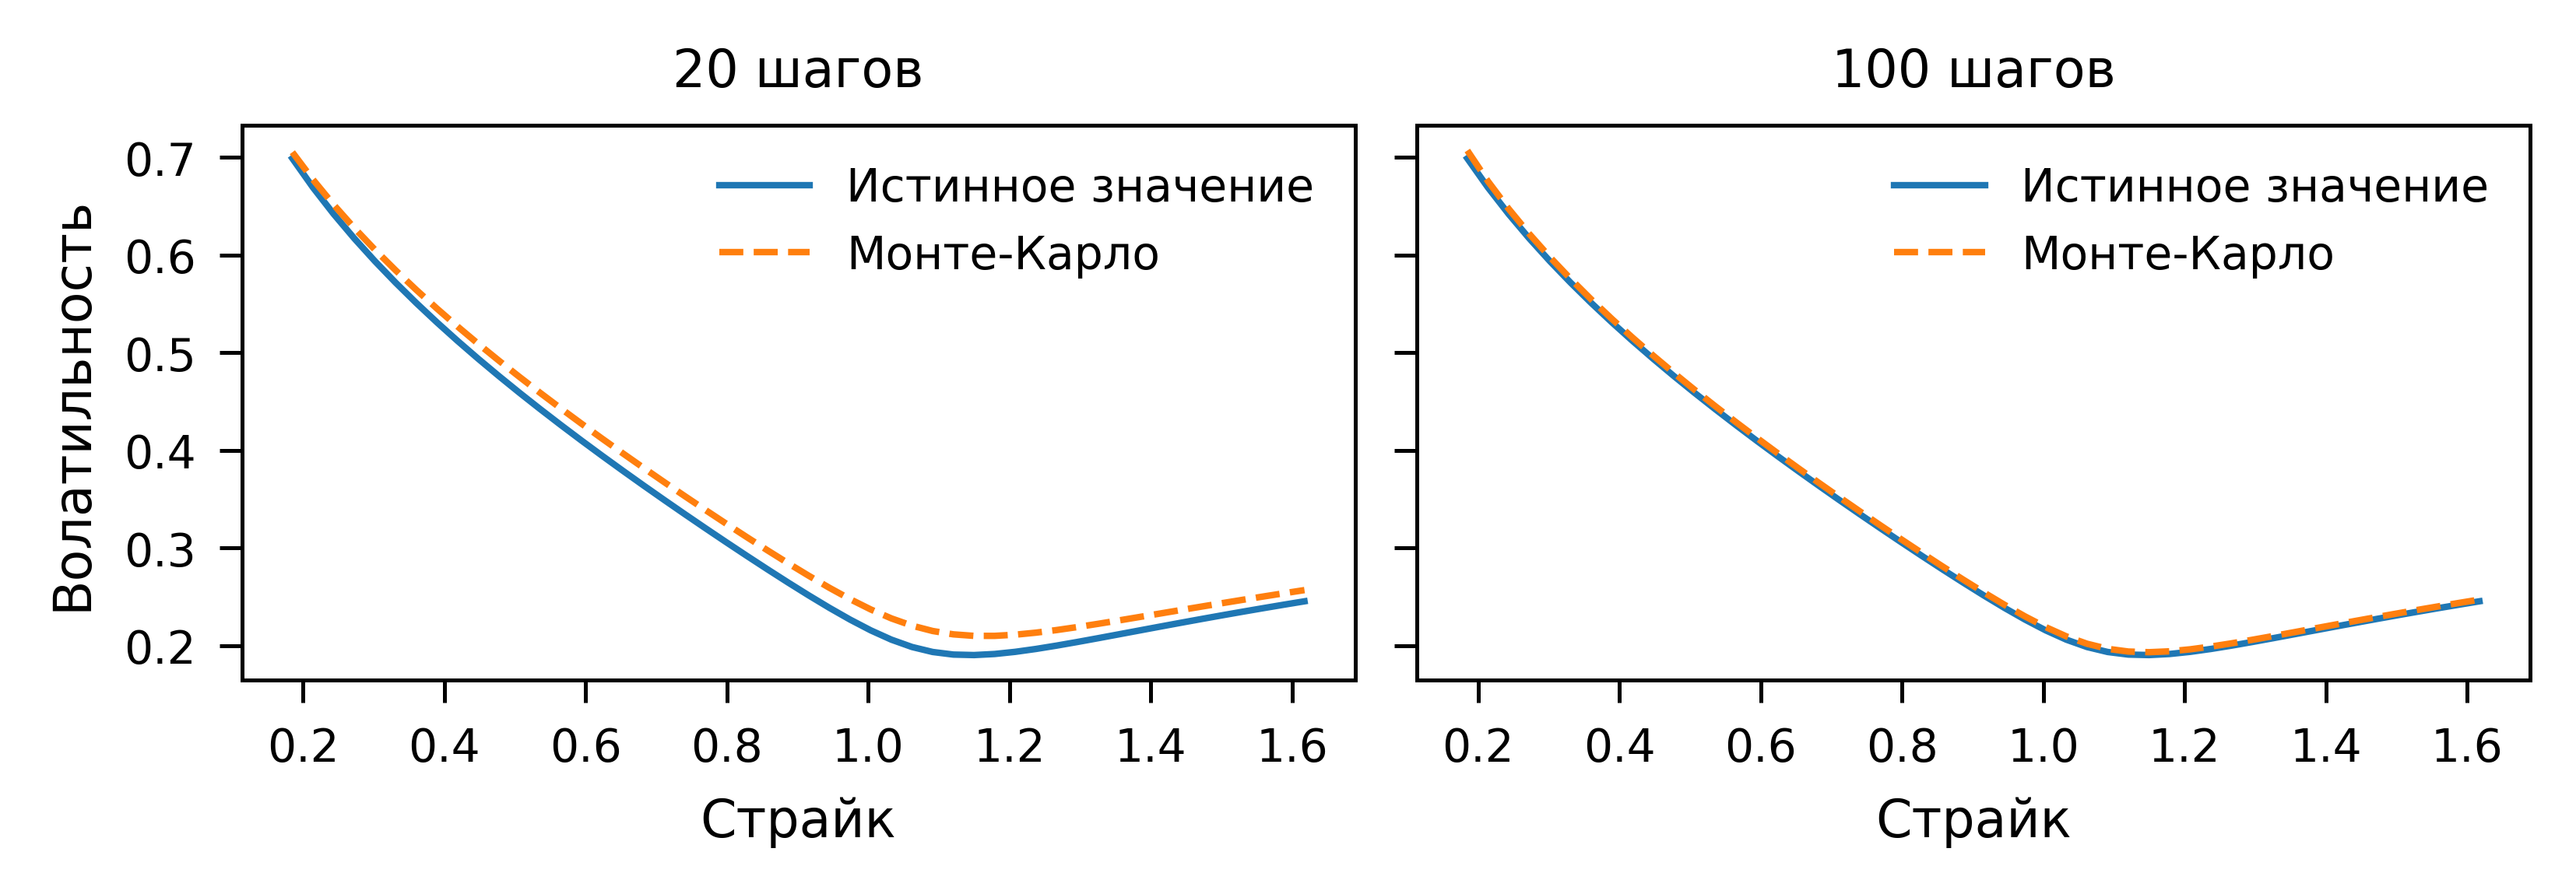
\includegraphics{pic/heston-euler.png}
\caption{Сходимость схемы Эйлера для модели Хестона.}
\label{hdg:f:euler}
\end{figure}


\summary
\begin{itemize}
\item В модели Хестона цены платежных обязательств, не зависящих от траектории цены базового актива, удовлетворяют дифференциальному уравнению с частными производными \eqref{hdg:pde}--\eqref{hgd:pde-boundary}.

\item Становится возможным реплицировать платежные обязательства, если добавить в портфель какое-нибудь дополнительно торгуемое платежное обязательство (например, опцион колл или пут).

\item Цены платежных обязательств можно вычислять с помощью метода \mc.
Для симуляции случайных процессов их траектории нужно дискретизировать.
В лекции рассматривалась схема дискретизации Эйлера.

\item Схема Эйлера имеет сильный порядок сходимости 1/2 и слабый порядок сходимости 1.
\end{itemize}
